\section{Results}
\label{sec:results}
Each of the following topics presents the results of the subsections discussed in Section~\ref{sec:methodology}.

\subsubsection{Project Builds}
As mentioned in Subsection~\ref{sec:methodology:sub:dataset}, only 19 out of the 21 projects contained in BugOSS could be successfully built. These projects were then used with the static analyzers. The fact that not all projects could be built points to a flaw in BugOSS regarding reproducibility.

\subsubsection{Static Analysis Results}
To evaluate the detection capabilities of the static analysis tools, both CodeQL and Infer were run on the 19 successfully built projects. The number of flagged vulnerabilities for each project is summarized in Table~\ref{sast_results}. It is important to denote that Infer could not be executed on Harfbuzz due to its unsupported build system.

\begin{table}[ht]
\centering
\caption{Number of vulnerabilities flagged by CodeQL and Infer for each project.}
\label{sast_results}
\begin{tabular}{|l|c|c|}
\hline
\textbf{Project Name} & \textbf{Flagged by CodeQL} & \textbf{Flagged by Infer} \\
\hline
Arrow & 0 & 71 \\
Aspell & 0 & 63 \\
Curl & 5 & 33 \\
Exiv2 & 3 & 55 \\
File & 0 & 107 \\
Gdal & 152 & 876 \\
Grok & - & - \\
Harfbuzz & 0 & - \\
Leptonica & 1 & 200 \\
Libarchive & 2 & 200 \\
Libhtp & 1 & 15 \\
Libxml2 & - & - \\
Ndpi & 5 & 75 \\
Openh264 & 11 & 191 \\
OpenSSL & 55 & 200 \\
PcapPlusPlus & 1 & 51 \\
Poppler & 15 & 200 \\
Readstat & 3 & 66 \\
Usrsctp & 2 & 0 \\
Yara & 1 & 24 \\
Zstd & 2 & 20 \\
\hline
Total & \textbf{259} & \textbf{2447} \\
\hline
\end{tabular}
\end{table}

As shown in the table, CodeQL flagged significantly fewer vulnerabilities compared to Infer. While Infer specializes in detecting memory-related vulnerabilities, CodeQL's default query set focuses on issues like SQL injection and cross-site scripting, which are uncommon in this dataset. CodeQL's analysis could possibly be improved with customized queries adapted to the nature of the projects in question.

The high amounts of flagged vulnerabilities by Infer is a great example as to why SAST tools present a challenge for a very effective and seamless continuous use. Sifting through so many warnings, searching for true positives, proves to be very strenuous and time-consuming for developers. The approach presented in this paper hopes to reduce the number of warnings which would then need to be manually checked.

\subsubsection{Gathering Contextual Information}
As previously mentioned 9, of the vulnerabilities flagged by Infer were found in the call graph and used for analysis in this step. Table~\ref{context} provides an overview of how many callers and callees each of the 9 functions had.

\begin{table}[ht]
\centering
\caption{Number of relevant callers and callees found per function analyzed.}
\label{context}
\begin{tabular}{|l|c|c|}
\hline
\textbf{Function} & \textbf{\#Callers} & \textbf{\#Callees} \\
\hline
light\_create\_default\_file\_info & 1 & 0 \\
light\_create\_file\_info & 1 & 0 \\
light\_pcapng\_open\_read & 1 & 0 \\
light\_pcapng\_open\_write & 2 & 0 \\
pcpp::IDnsResource::decodeName & 1 & 4 \\
pcpp::IDnsResource::encodeName & 2 & 4 \\
pcpp::IPFilter::convertToIPAddressWithLen & 1 & 13 \\
pcpp::IPv4Layer::parseNextLayer & 8 & 37 \\
pcpp::IPv6Layer::parseExtensions & 3 & 11 \\
\hline
\end{tabular}
\end{table}

It is important to note that function calls pertaining to the C/C++ standard libraries, the LLVM compiler or any other compilation step, like an address sanitizer, that did not correspond to a function in the PcapPlusPlus repository, were not considered in this analysis, since they went out of the scope of the project.

As explained in Subsections~\ref{sec:methodology:sub:context} and~\ref{sec:methodology:sub:llm}, the source code for all these functions was gathered in separate files, whose paths were then given in the prompt.

\subsubsection{LLM Analysis}
Figure~\ref{chart} depicts the results of the LLM analysis by showing how the 51 functions examined fared in terms of false or true positives.
Regarding these results, there are some interesting points which must be addressed:

\begin{figure}[ht]
    \centering
    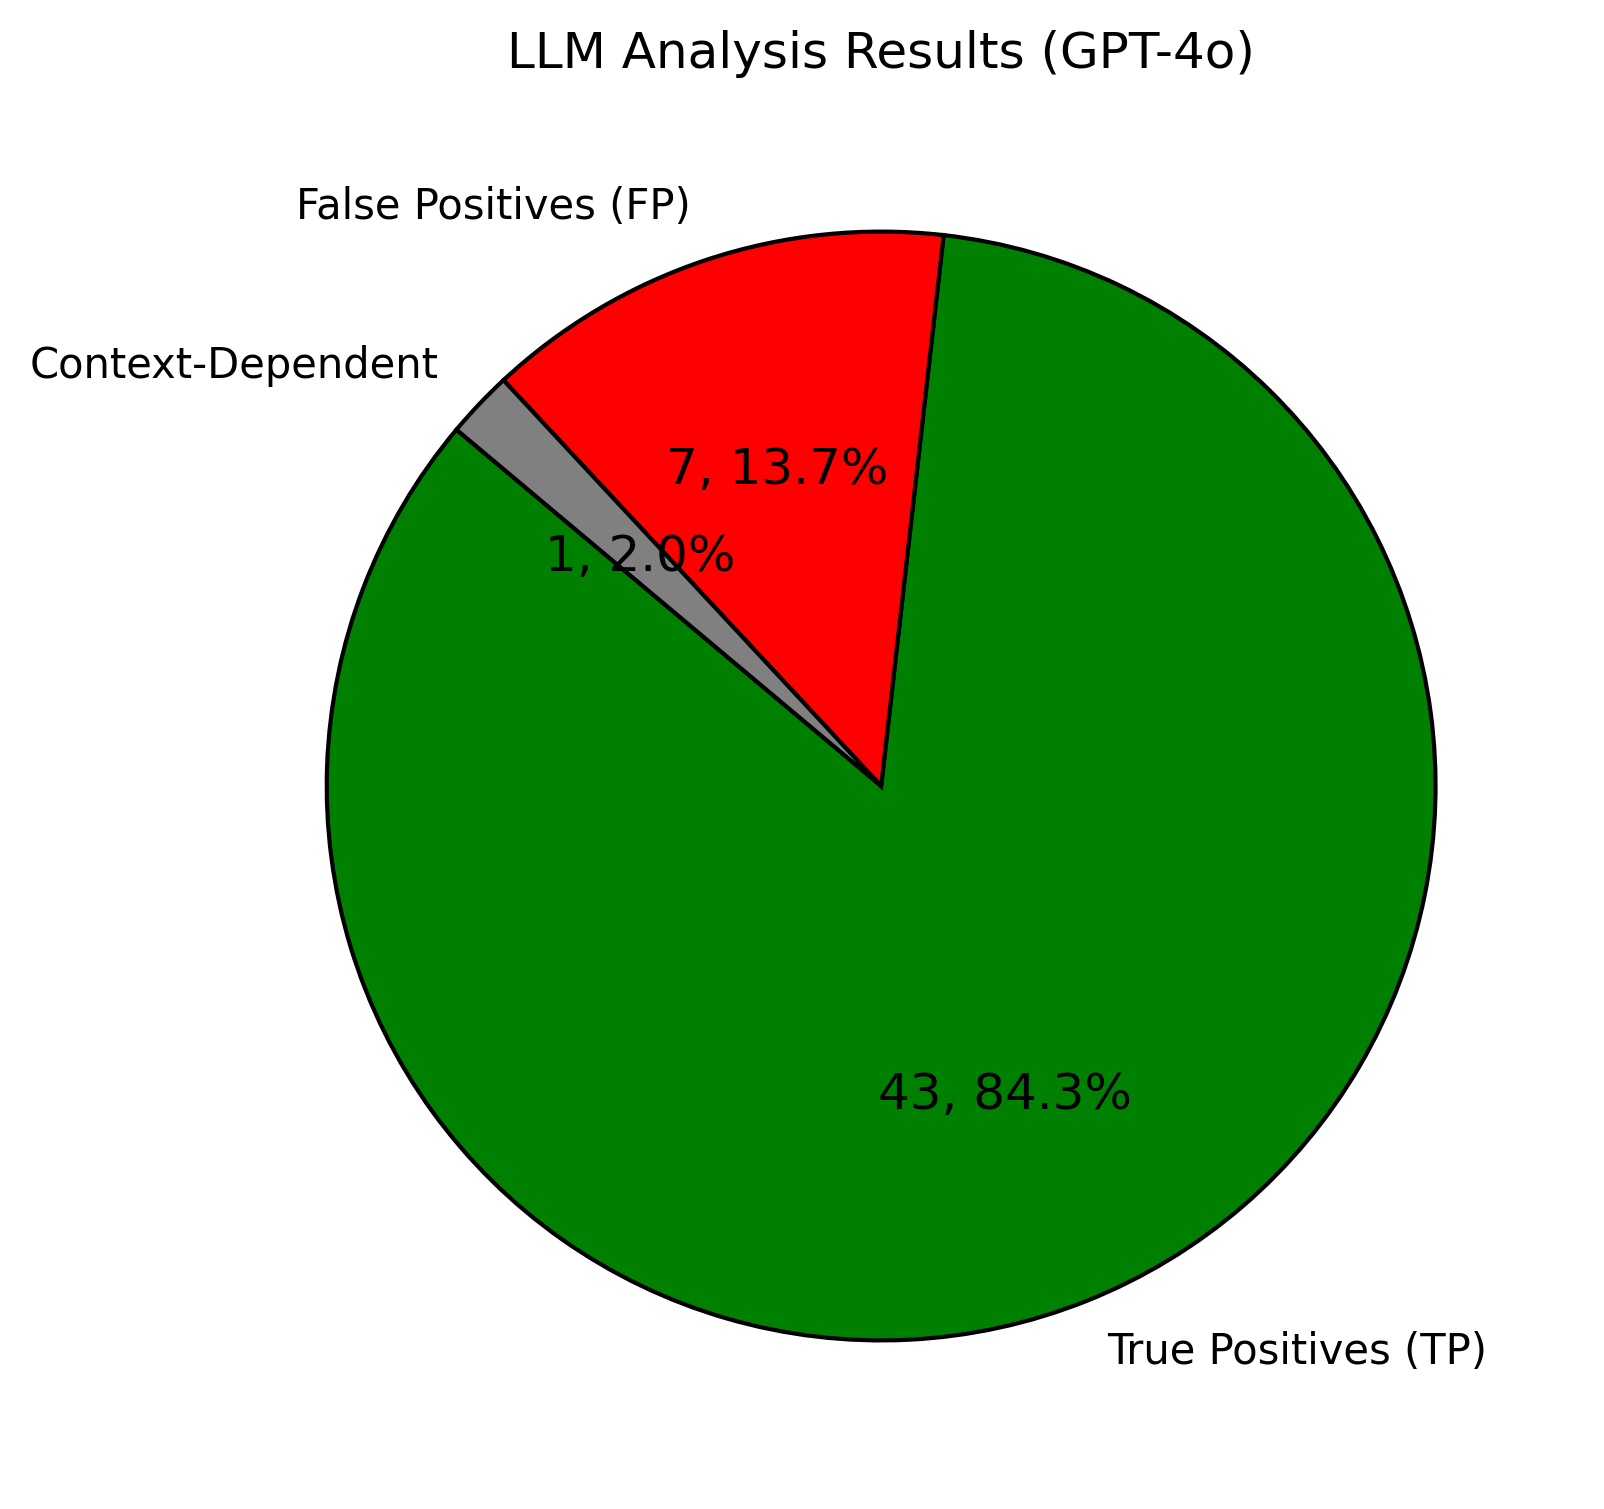
\includegraphics[scale=0.7]{figures/llm_analysis_results_with_numbers.png} 
    \caption{Results of the analysis with GPT-4o.}
    \label{chart}
\end{figure}

\begin{itemize}
    \item For one of the functions, marked in gray, the LLM did not provide a definitive answer as to whether the flagged vulnerability was a true or a false positive. Instead, it affirmed that information regarding one specific callee of the function would be necessary to come to a decision. This one callee was supposedly responsible for assigning NULL values to some fields in the data structure, which would then lead to a NULL dereference error if unchecked. Unfortunately, this callee was not picked up by SVF in the previous step, so the LLM lacked the context in this case.
    \item Many of the vulnerabilities flagged by Infer consisted in NULL dereferences, which usually appeared in the form of pointers to freshly allocated memory not being immediately checked. This type of issue is one which does not require much reasoning to correctly identify, but rather just looking for a NULL check after the allocation.
    \item Most interesting was GPT-4o's analysis of the ground truth vulnerability. As previously explained, the ground truth was considered found if the SAST tools marked any possible errors inside the same function. In the case of PcapPlusPlus, the actual problem is a buffer overflow, which happens a few lines before the dead store marked by Infer. After looking through the source code, the LLM decided that the flagged issue was a false positive, as the variable was used in pointer arithmetic. But following this verdict, it mentioned a "potential buffer issue" and pointed to the line of the ground truth, correctly explaining the reason for the vulnerability.
\end{itemize}

Table~\ref{fps} shows, for each of the 9 functions whose context could be gathered, whether GPT-4o flagged the issue as a false (FP) or true positive (TP), and the type of vulnerability originally marked by Infer. For further analysis, these functions were manually inspected to qualitatively evaluate the LLM's assessment.
\begin{table}[ht]
\centering
\caption{Qualitative Analysis from the LLM.}
\label{fps}
\begin{tabular}{|l|c|c|}
\hline
\textbf{Function} & \textbf{Verdict} & \textbf{Issue Type} \\
\hline
light\_create\_default\_file\_info & TP & NULL\_DEREFERENCE \\
light\_create\_file\_info & TP & NULL\_DEREFERENCE \\
light\_pcapng\_open\_read & TP & NULL\_DEREFERENCE \\
light\_pcapng\_open\_write & TP & NULL\_DEREFERENCE \\
pcpp::IDnsResource::decodeName & FP & DEAD\_STORE \\
pcpp::IDnsResource::encodeName & FP & DEAD\_STORE \\
pcpp::IPFilter::convertToIPAddressWithLen & TP & DEAD\_STORE \\
pcpp::IPv4Layer::parseNextLayer & TP & DEAD\_STORE \\
pcpp::IPv6Layer::parseExtensions & TP & NULL\_DEREFERENCE \\
\hline
\end{tabular}
\end{table}

As just mentioned, NULL\_DEREFERENCE issues do not require much reasoning. In the case of these functions, it was clear that there was no check after the memory allocations or function calls which changed the flagged pointers.

Regarding the DEAD\_STORE issues, there are some interesting observations, after human inspection of the warnings is done:
\begin{itemize}
    \item For decodeName, GPT-4o outputs, in its conclusion: "The flagged issue appears to be a false positive in terms of security, as decodedNameLength is not used in a way that introduces a vulnerability. However, the presence of the variable as a dead store is indicative of inefficient or unclear code, and removing or repurposing it could improve maintainability.". So, despite detecting an unused value and agreeing with the static analysis result, which is incorrect after manually analyzing the code, the model correctly phrases it as it not actually being a true positive. 
    \item In regards to encodeName, the LLM recognizes the argument flagged by Infer as a pointer which is modified, not needing to be assigned to another variable or returned for it to be considered "used".
    \item Contrary to the previous point, GPT-4o does not recognize the flagged variables in convertToIPAddressWithLen as ones modifying a memory address, which is then later used.
    \item The LLM marks the issues in parseNextLayer as true positives. However, the flagged variables are clearly used, after manual inspection, for choosing which types of layers to instantiate.
\end{itemize}

The observations above highlight the fact that there is still room for improvement regarding the model's reasoning capabilities. The outputs were correct for the most simple type of issue, the null dereference, but not for the ones which demanded greater comprehension of the code.
The LLM did, however, also show promise by correctly identifying the ground truth vulnerability, despite the issue flagged by Infer being unrelated to it.